% Copyright 2004 by Till Tantau <tantau@users.sourceforge.net>.
%
% In principle, this file can be redistributed and/or modified under
% the terms of the GNU Public License, version 2.
%
% However, this file is supposed to be a template to be modified
% for your own needs. For this reason, if you use this file as a
% template and not specifically distribute it as part of a another
% package/program, I grant the extra permission to freely copy and
% modify this file as you see fit and even to delete this copyright
% notice. 

\documentclass[mathserif, xcolor=table]{beamer}
\usepackage{url}
\usepackage{hyperref}
\usepackage{caption}
\usepackage[round]{natbib}
\usepackage{graphicx}
\usepackage{subcaption}
\usepackage{multicol}
\usepackage{multirow}
\usepackage{booktabs}
\usepackage{dcolumn}
\usepackage{tikz}
\usepackage{amssymb}
\usepackage{natbib}
\usetikzlibrary{graphs,decorations.pathreplacing}

\setbeamertemplate{caption}[numbered]

% There are many different themes available for Beamer. A comprehensive
% list with examples is given here:
% http://deic.uab.es/~iblanes/beamer_gallery/index_by_theme.html
% You can uncomment the themes below if you would like to use a different
% one:
\usetheme{AnnArbor}
%\usetheme{Antibes}
%\usetheme{Bergen}
%\usetheme{Berkeley}
%\usetheme{Berlin}
%\usetheme{Boadilla}
%\usetheme{boxes}
%\usetheme{CambridgeUS}
%\usetheme{Copenhagen}
%\usetheme{Darmstadt}
%\usetheme{default}
%\usetheme{Frankfurt}
%\usetheme{Goettingen}
%\usetheme{Hannover}
%\usetheme{Ilmenau}
%\usetheme{JuanLesPins}
%\usetheme{Luebeck}
%\usetheme{Madrid}
%\usetheme{Malmoe}
%\usetheme{Marburg}
%\usetheme{Montpellier}
%\usetheme{PaloAlto}
%\usetheme{Pittsburgh}
%\usetheme{Rochester}
%\usetheme{Singapore}
%\usetheme{Szeged}
%\usetheme{Warsaw}
%\useoutertheme{infolines}
%\useinnertheme{rectangles}
\usecolortheme{crane}
% https://en.wikibooks.org/wiki/LaTeX/Presentations

%\definecolor{UTDOrange}{RGB}{223,117,0} 
%\definecolor{UTDGreen}{RGB}{18,71,52}

%\setbeamercolor{palette primary}{bg=UTDOrange,fg=white}
%\setbeamercolor{palette secondary}{bg=UTDOrange,fg=white}
%\setbeamercolor{palette tertiary}{bg=UTDOrange,fg=white}
%\setbeamercolor{palette quaternary}{bg=UTDOrange,fg=white}
%\setbeamercolor{section in toc}{fg=black} % TOC sections

%\setbeamercolor{title}{fg=black, bg=UTDOrange}
%\setbeamercolor{titlelike}{fg=black, bg=UTDOrange}

% Override palette coloring with secondary
%\setbeamercolor{subsection in head/foot}{bg=UTDGreen,fg=white}

\title{Value Of Local Showrooms To Online Competitors}

% A subtitle is optional and this may be deleted
\subtitle{Causal Forest Application with R}

\author{\textbf{Author}: Jayarajan Samuel, Zhiqiang (Eric) Zheng, Ying Xie \\ 
{\footnotesize \textbf{Group Members}: Beyza Celik, Luoying Chen, Yihong Liu, Duc Vu}}

% - Give the names in the same order as the appear in the paper.
% - Use the \inst{?} command only if the authors have different
%   affiliation.

\institute[] % (optional, but mostly needed)
{  
%  \inst{1}%
%  Marketing \\ London Business School
%  
%  \inst{2}%
%  Marketing \\ Massachusetts Institute of Technology
%  
%  \inst{3}%
%  Naveen Jindal School of Management \\ University of Texas at Dallas \\ \url{https://liu-yihong.github.io/}
}
% - Use the \inst command only if there are several affiliations.
% - Keep it simple, no one is interested in your street address.

\date{October 23, 2020}
% - Either use conference name or its abbreviation.
% - Not really informative to the audience, more for people (including
%   yourself) who are reading the slides online

% \subject{Management Science}
% This is only inserted into the PDF information catalog. Can be left
% out. 

% If you have a file called "university-logo-filename.xxx", where xxx
% is a graphic format that can be processed by latex or pdflatex,
% resp., then you can add a logo as follows:

\pgfdeclareimage[height=0.9cm]{university-logo}{figures/header-JSOM-Black2.png}
\logo{\pgfuseimage{university-logo}}

% Delete this, if you do not want the table of contents to pop up at
% the beginning of each subsection:

%\AtBeginSubsection[]
%{
%  \begin{frame}<beamer>{Outline}
%    \tableofcontents[currentsection,currentsubsection]
%  \end{frame}
%}

%gets rid of bottom navigation bars
\setbeamertemplate{footline}[page number]{}

%gets rid of navigation symbols
\setbeamertemplate{navigation symbols}{}

% Let's get started
\begin{document}

\begin{frame}
  \titlepage
\end{frame}

% \begin{frame}[allowframebreaks]{Outline}
%   \tableofcontents
%   % You might wish to add the option [pausesections]
% \end{frame}

% \section{Background}
% \begin{frame}[allowframebreaks]{Background}
% 	\begin{itemize}
% 		\item Online Shopping vs Offline
% 		\begin{multicols}{2}
% 			\begin{itemize}
% 				\item Online Info Hub
% 				\begin{enumerate}
% 					\item Usually lower price
% 					\item Various types
% 					\item Less time
% 				\end{enumerate}
% 				\item Offline Showroom
% 				\begin{enumerate}
% 					\item Physically experienced
% 					\item Real-time assistance
% 					\item Instant gratification
% 				\end{enumerate}
% 			\end{itemize}
% 		\end{multicols}
% 		\item Customer interacts between online and offline
% 	\end{itemize}
% 	\framebreak
% % 	\begin{figure}[h]
% % 		\centering
% % 		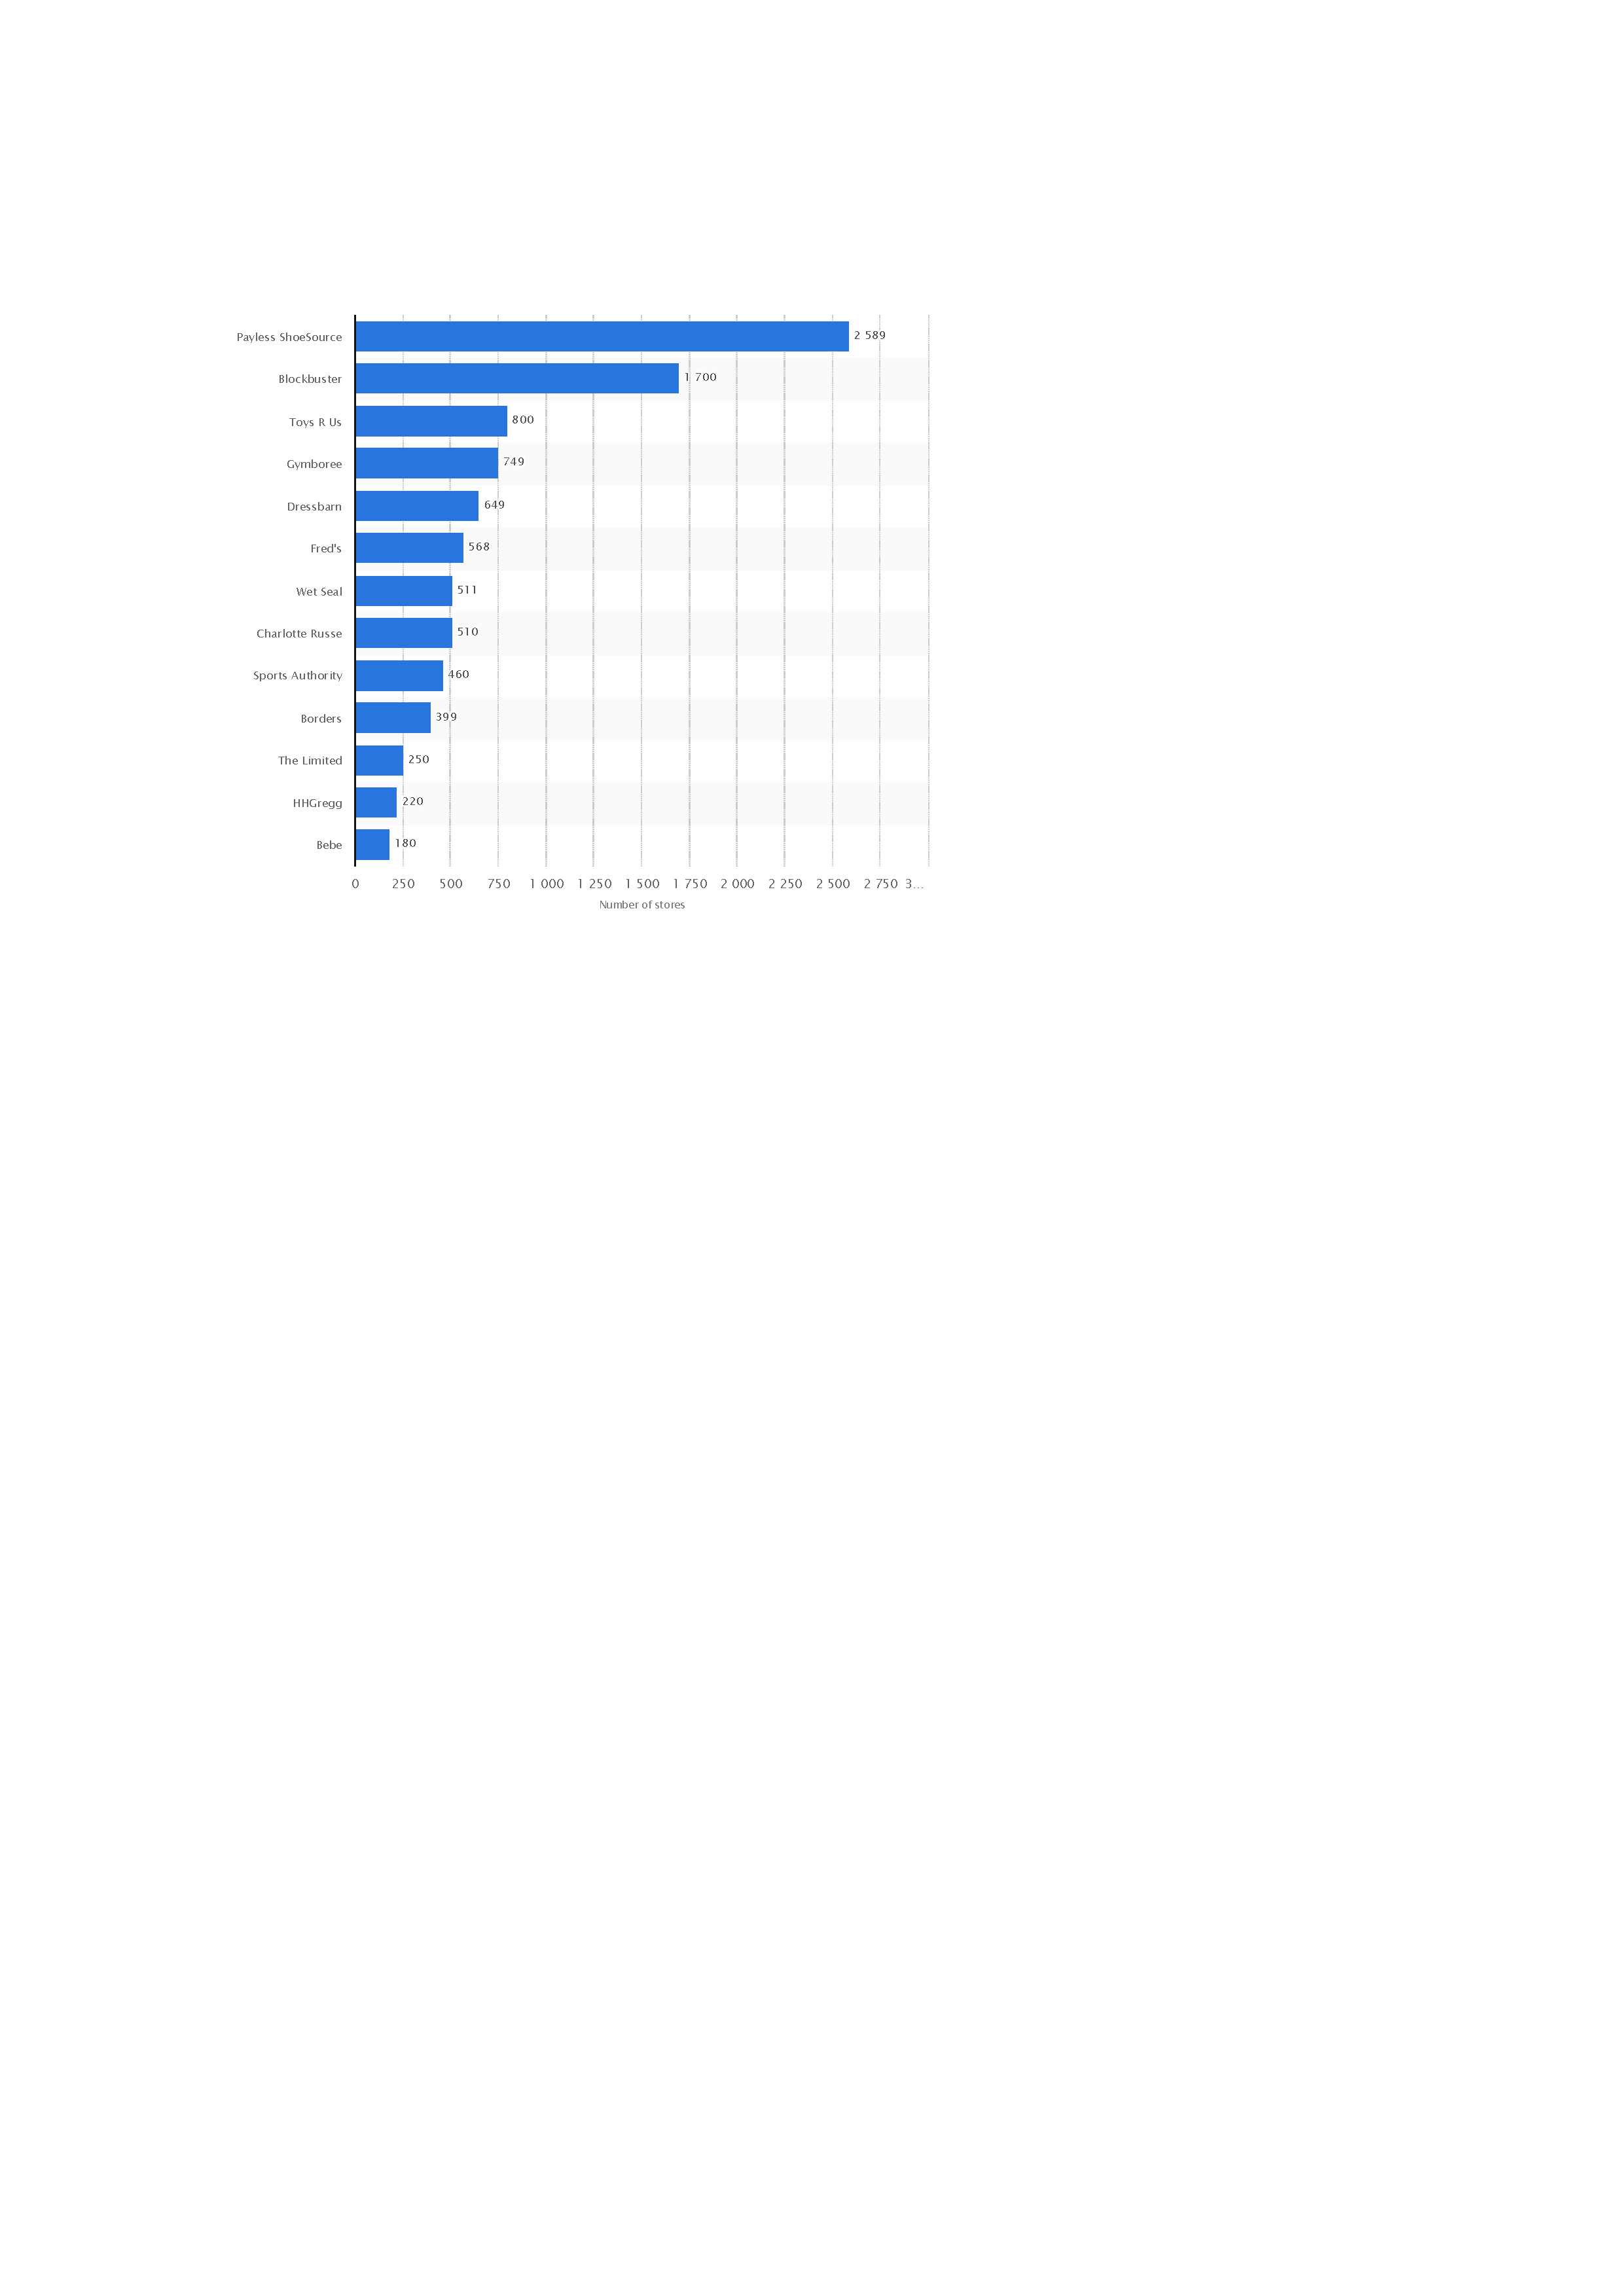
\includegraphics[scale=0.3]{pic/retail_closure.pdf}
% % 		\caption{Num Of Store Closures by Selected Retailers in US From 2010 to 2020 \footnote{\href{https://www.statista.com/statistics/1092243/number-of-stores-closures-by-selected-retailers-us/}{source link: statista.com}}}
% % 	\end{figure}
% 	\begin{itemize}
% 		\item Values of offline store closures for online retailers?
% 	\end{itemize}
% \end{frame}
\section{Introduction}
\begin{frame}{Data Preparation for the Application}
\begin{itemize}
    \item Our analysis is based on data individual transactions. 
    \item For each transaction $i=1,\dots,n$,
    \begin{itemize}
        \item $W_i=\texttt{CCStorePresent}_i\times\texttt{AfterStoreClosing}_i$
        \item $Y_i=\log\left(\texttt{prod\_totprice},\;\texttt{PagesPerDollar},\;\texttt{MinsPerDollar}\right)$ \footnote{right-skewed}
        \item  \textbf{10 categorical}: \texttt{hoh\_most\_education}, \texttt{census\_region}, \texttt{household\_size}, \texttt{hoh\_oldest\_age}, \texttt{children}, \texttt{racial\_background}, \texttt{connection\_speed}, \texttt{country\_of\_origin}, \texttt{prod\_category\_type} and \texttt{BBStorePresent}
        \item \textbf{4 real-valued covariates}: \texttt{pages\_viewed}\footnote{not \texttt{PagesPerDollar} is dependent variable}, \texttt{duration}\footnote{not \texttt{MinsPerDollar} is dependent variable}, \texttt{prod\_qty}, \texttt{household\_income}
        \item We expanded out categorical random variables via one-hot encoding, thus resulting in covariates $X_i \in \mathbb{R}^p$  with $p = 38$ or $p = 37$ .
    \end{itemize}
\end{itemize}

\end{frame}
\section{Causal Forest Algorithm}
\begin{frame}[allowframebreaks]{The potential outcomes framework}
For a set of i.i.d. subjects $i = 1, ..., n$, we observe a tuple $(X_i , Y_i , W_i )$, comprised of
\begin{itemize}
    \item A \textbf{feature vector} $X_i \in \mathbb{R}^p,$
    \item A \textbf{response} $Y_i \in \mathbb{R}$, and 
    \item A \textbf{treatment assignment} $W_i \in \{0,1\}$\\~
\end{itemize}

Following the \textbf{potential outcomes} framework \citep{imbens2015causal} , we posit the existence of quantities $Y_i(0)$ and $Y_i(1)$ 

\begin{itemize}
    \item These correspond to the response we would have measured given that the $i$-th subject received treatment ($W_i = 1$) or no treatment ($W_i = 0$).
\end{itemize}
\framebreak
Goal is to estimate the \textbf{conditional average treatment effect}
\begin{equation*}
    \tau(x)=\mathbb{E}\left[Y(1)-Y(0)\mid X=x\right]
\end{equation*}
However in experiments we only get to see $Y_i=Y_i(W_i)$

\framebreak

If we make no further assumptions, estimating $\tau(x)$ is not possible. 
\begin{itemize}
    \item Literature often assumes \textbf{unconfoundedness} \citep{rosenbaum1983central}
\begin{equation*}
    \{Y_i(0), Y_i(1)\}\perp \!\!\! \perp W_i \mid X_i.
\end{equation*}
    \item When this assumption holds, methods based on matching or propensity score estimation are usually consistent. 
\end{itemize}
\end{frame}



% \begin{frame}{Classification Trees: Titanic Example}
% \begin{figure}[h]
%     \centering
%     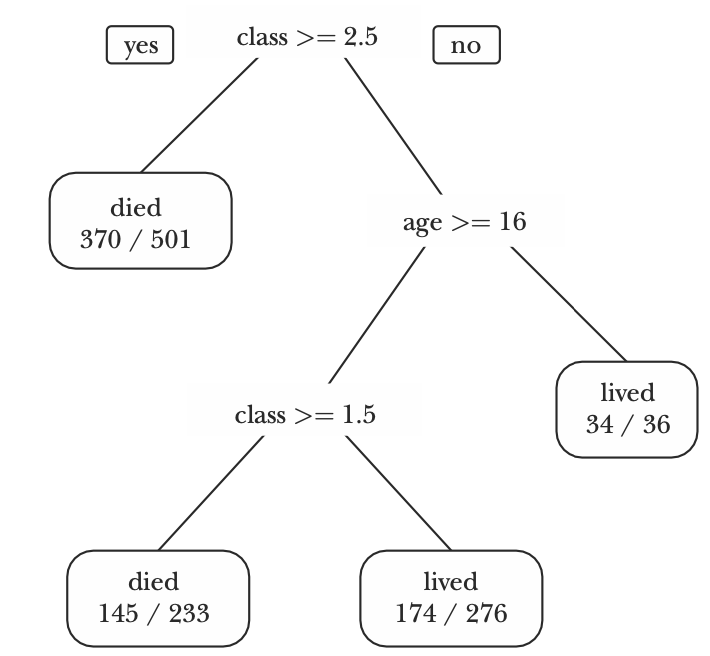
\includegraphics[scale=0.45]{figures/titanic.png}
%     \caption{A Classification Tree for Survivors of the Titanic \footnote{\citep{varian2014big}}}
%     \label{fig:titanic}
% \end{figure}
% \end{frame}

% \begin{frame}{Regression Trees: The Tree as a Partition}
% \begin{figure}[h]
%     \centering
%     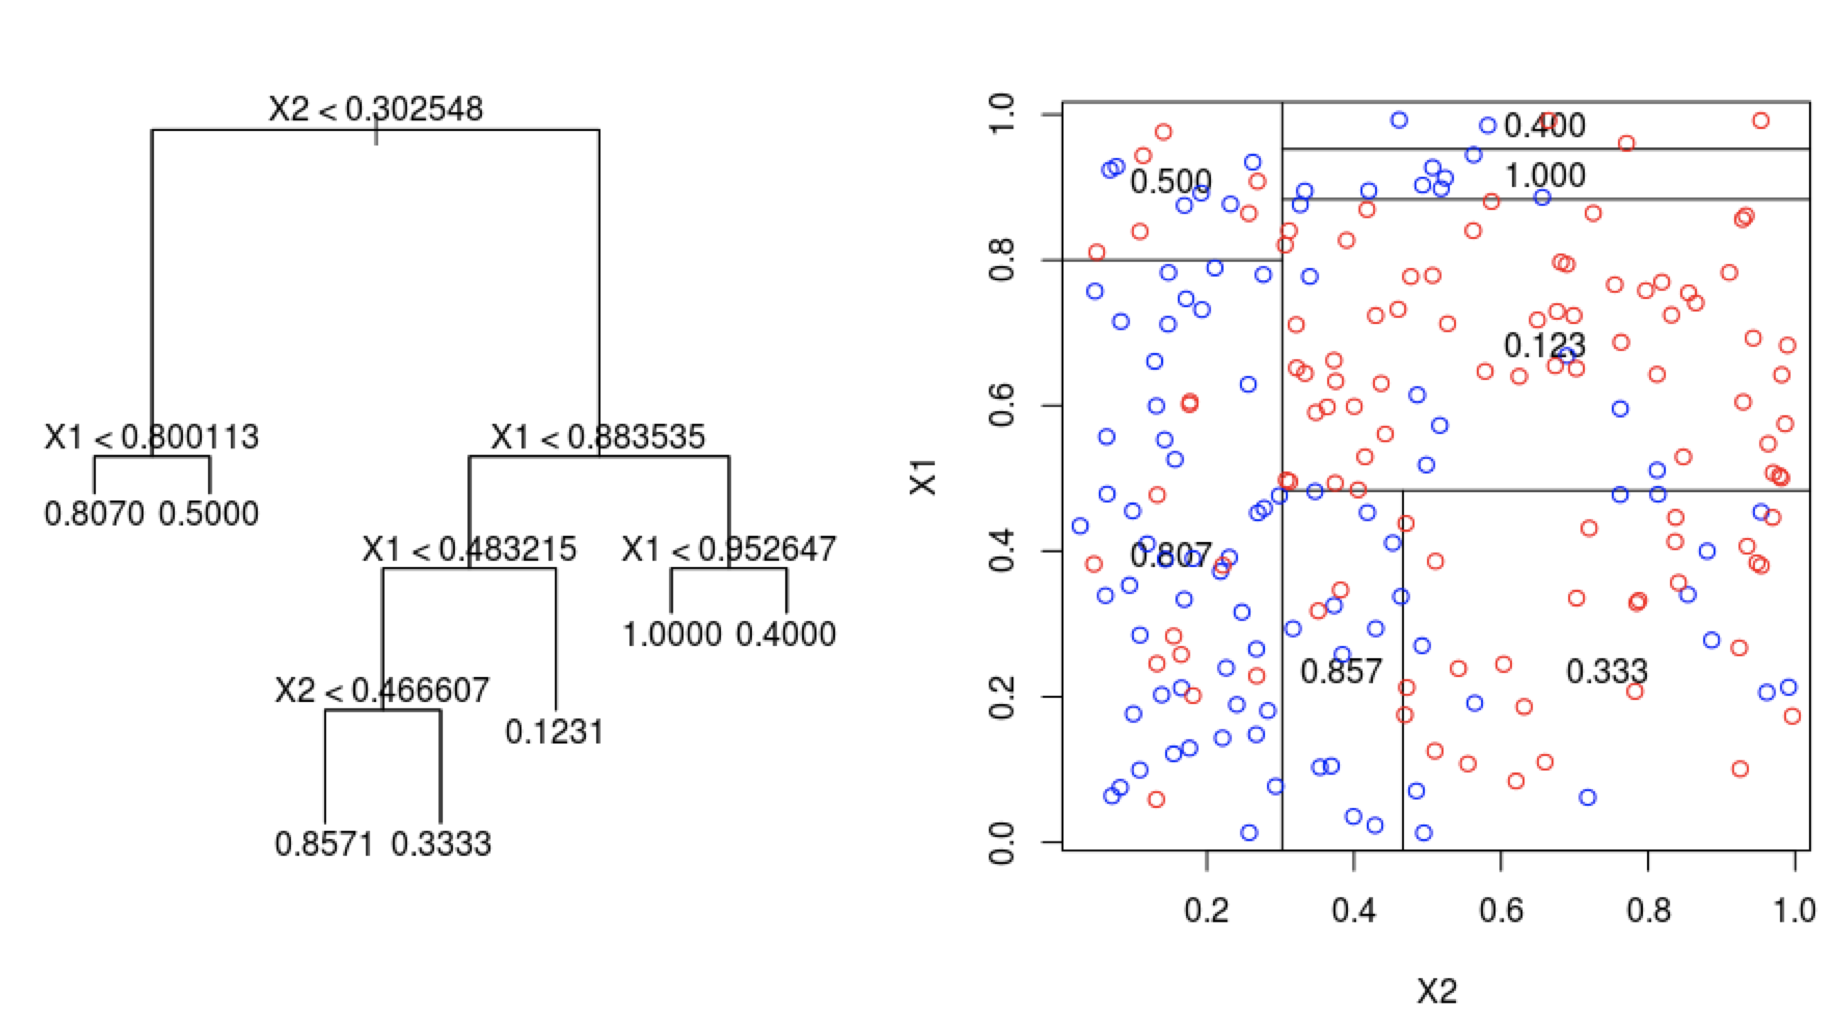
\includegraphics[scale=0.3]{figures/regression_tree.png}
%     \caption{A Regression Tree Example}
%     \label{fig:regress_tree}
% \end{figure}
% \end{frame}

% \begin{frame}{Causal Trees}
% % % Causal Tree Learning, a machine learning technique developed by the economists Susan Athey and Guido Imbens for automatically estimating heterogeneous treatment effects conditional on a large number of confounding variables. Causal Tree Learning leverages a machine learning algorithm known as decision tree learning to identify an optimal strategy for splitting observed individuals into groups to estimate heterogeneous treatment effects. (Divide population into subgroups to minimize MSE in treatment effects)
% % How can decision trees help an analyst estimate heterogeneous treatment effects?
% % % Decision trees used for these traditional inference tasks generally estimate a function mapping characteristics about individuals to the value of a target variable, such as the decision tree presented in Figure \ref{fig:titanic}, which maps information about passengers on the Titanic to their probability of surviving its crash. Adversely, decision trees for causal inference are generally used to separate data into buckets, in order to enable a calculation estimating average treatment effects within each node. The process of decision tree learning for causal inference can be separated into a step for each of these tasks, commonly referred to as the splitting step and the estimation step respectively.
% \begin{enumerate}
%     \item splitting step 
%     \item estimation step
% \end{enumerate}
% Difference from traditional decision tree learning algorithms:
% \begin{itemize}
%     \item splitting criterion -  $EMSE_{\tau}$ 
%     % expected mean squared error for treatment effects
%     \item honesty
% \end{itemize}
% % %Estimation step: This step consists of leveraging the decision tree estimated in the splitting step and using the tree from that step to split observed individuals according to the defined rules. As a result of this splitting, each leaf of the tree will consist of a group of similar observed individuals exposed and unexposed to treatment. Thus, to estimate the effect of treatment on observed individuals within each leaf, an analyst must simply calculate the difference in mean outcomes between those that have been exposed to treatment and those that have not. This calculation, the simple difference in mean outcomes of observed individuals within each leaf, is an unbiased CATE estimation conditional on the values of variables which define the leaf (the conditional statements on the path from this leaf to the root node).
% \end{frame}
\begin{frame}{Causal Forests for Observational Studies}
All analyses are carried out using the R package \textbf{grf}, version 1.2.0 \citep{tibshirani2018package}.
\begin{itemize}
    \item $e(x) = \mathbb{P}[W_i\mid X_i = x]$ for the propensity score 
    \item $m(x) = \mathbb{E}[Y_i\mid X_i = x]$ for the expected outcome marginalizing over treatment
    \item An application of causal forests using \textbf{grf} \citep{athey2019estimating}: 
    \begin{enumerate}
        \item fitting two separate regression forests to estimate $m(\cdot)$ and $e(\cdot)$ (\texttt{Y.forest} and \texttt{W.forest})
        \item It then makes out-of-bag predictions using these two first-stage forests, and uses them to grow a causal forest
        \item training a pilot random forest on all the features, and then train a second forest on only those features that saw a reasonable number of splits in the first step.
    \end{enumerate}
    \end{itemize}
\end{frame}

\section{Average Treatment Effect of Circuit City Stores Closure}
\begin{frame}{on amazon.com Sales}
% The first question asks about the overall effectiveness of the intervention. 
The package \textbf{grf} has a built-in function for average treatment effect estimation called \texttt{average\_treatment\_effect}. Using this function we obtain:
\vspace{-1em}
\begin{columns}
\begin{column}{.6\textwidth}
 \begin{figure}[h]
    \centering
    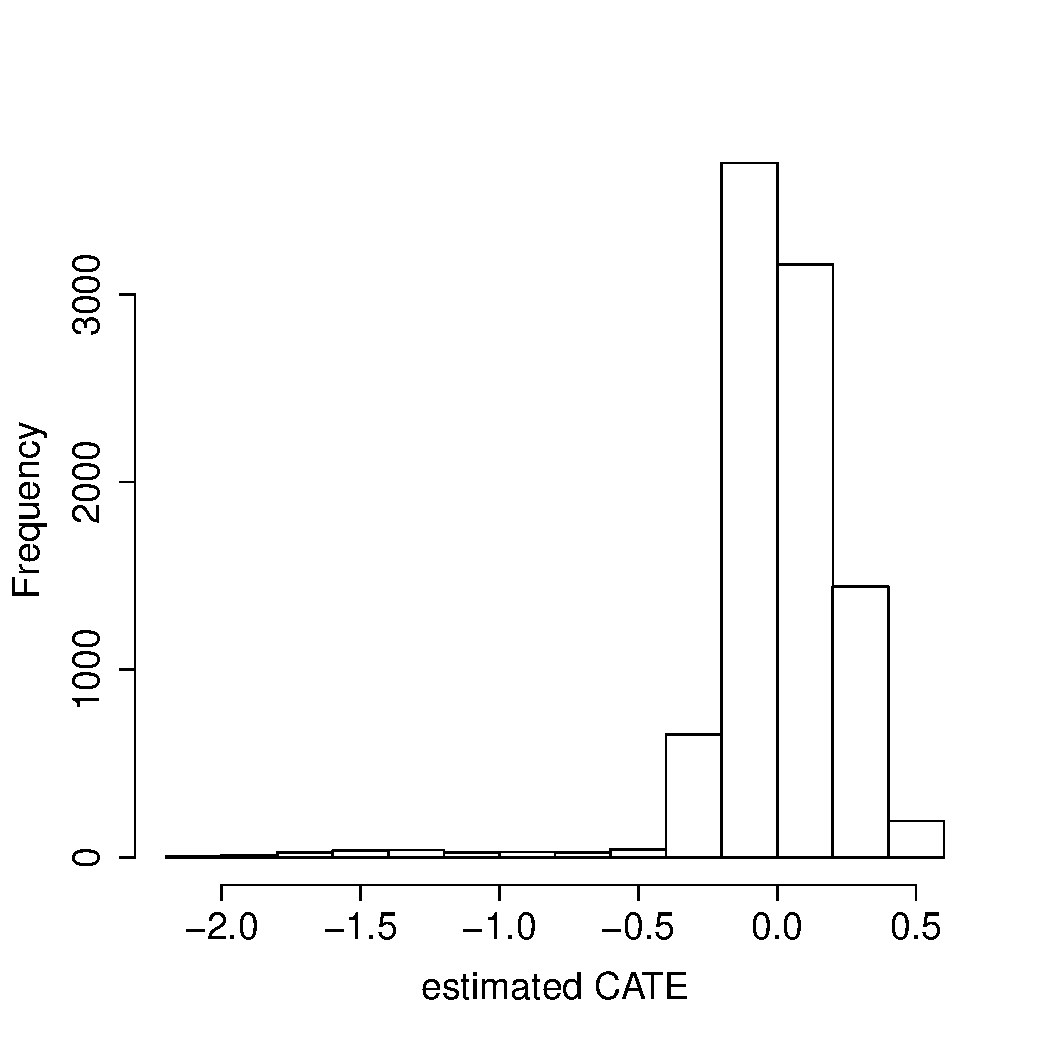
\includegraphics[scale=0.3]{figures/tauhat1_ama_hist.pdf}
    \caption{ Histogram of out-of-bag CATE estimates from a causal forest}
    \label{fig:tauhat1_ama_hist}
\end{figure}
 \end{column}

 \begin{column}{.39\textwidth}
 \begin{table}[h]
\label{}
\caption{90\% CI for the ATT}
\centering
\begin{tabular}{rrr}
  \hline
 5\%  & $\hat{\tau_t}$ & 95\% \\ 
  \hline
-0.42 & -0.22 & -0.03 \\ 
   \hline
\end{tabular}
 \end{table}
 \end{column}
\end{columns}
  \end{frame}

\begin{frame}{on bestbuy.com Sales}
% The first question asks about the overall effectiveness of the intervention. 
\vspace{-1em}
\begin{columns}
\begin{column}{.6\textwidth}
 \begin{figure}[h]
    \centering
    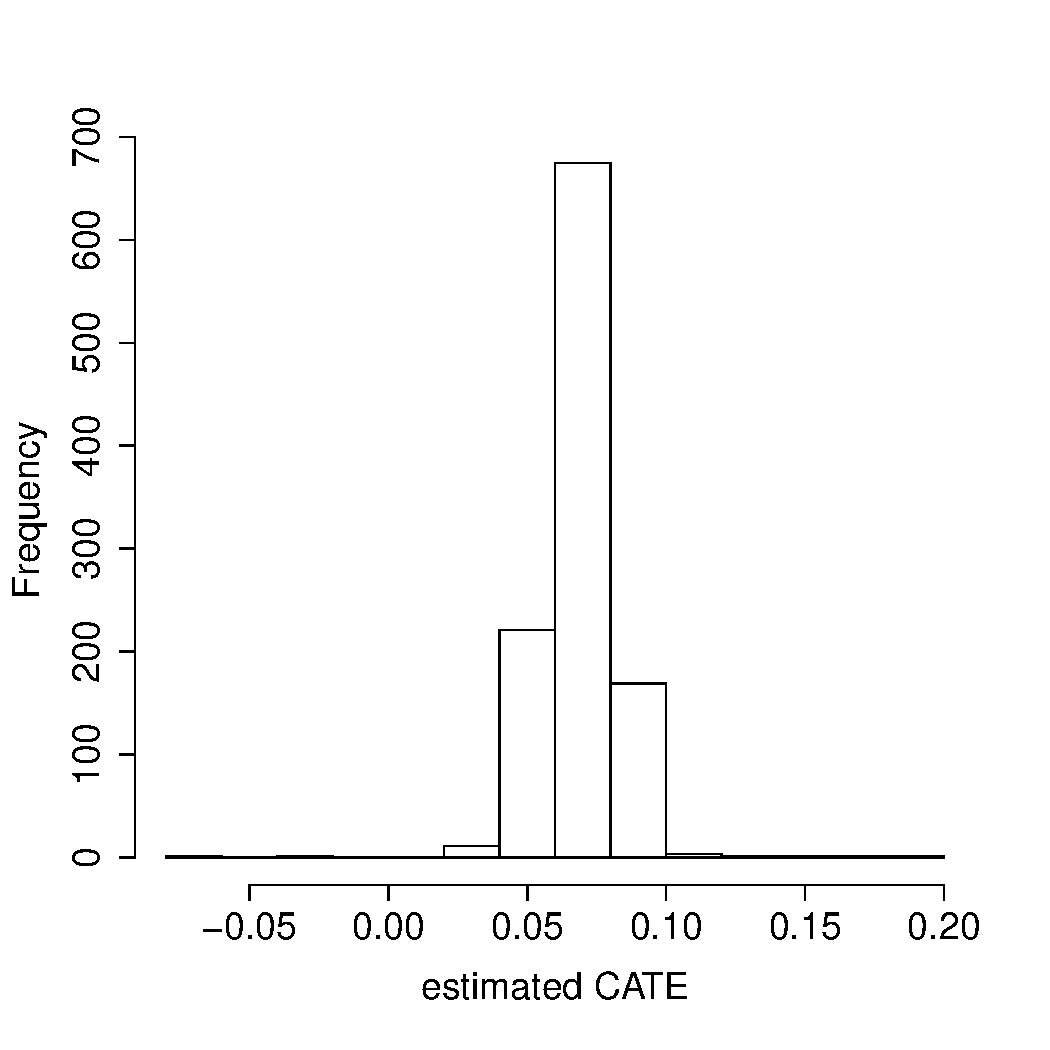
\includegraphics[scale=0.3]{figures/tauhat1_bb_hist.pdf}
    \caption{ Histogram of out-of-bag CATE estimates from a causal forest}
    \label{fig:tauhat1_bb_hist}
\end{figure}
 \end{column}

 \begin{column}{.39\textwidth}
 \begin{table}[h]
 \caption{90\% CI for the ATT} 
\centering
\begin{tabular}{rrr}
  \hline
 5\%  & $\hat{\tau_t}$ & 95\% \\ 
  \hline
 -0.39 & 0.08 & 0.55 \\ 
   \hline
\end{tabular}
\end{table}
 \end{column}
\end{columns}
\end{frame}
\begin{frame}{on amazon.com Pages Per Dollar of Sales}
% The first question asks about the overall effectiveness of the intervention. 
\vspace{-1em}
\begin{columns}
\begin{column}{.6\textwidth}
 \begin{figure}[h]
    \centering
    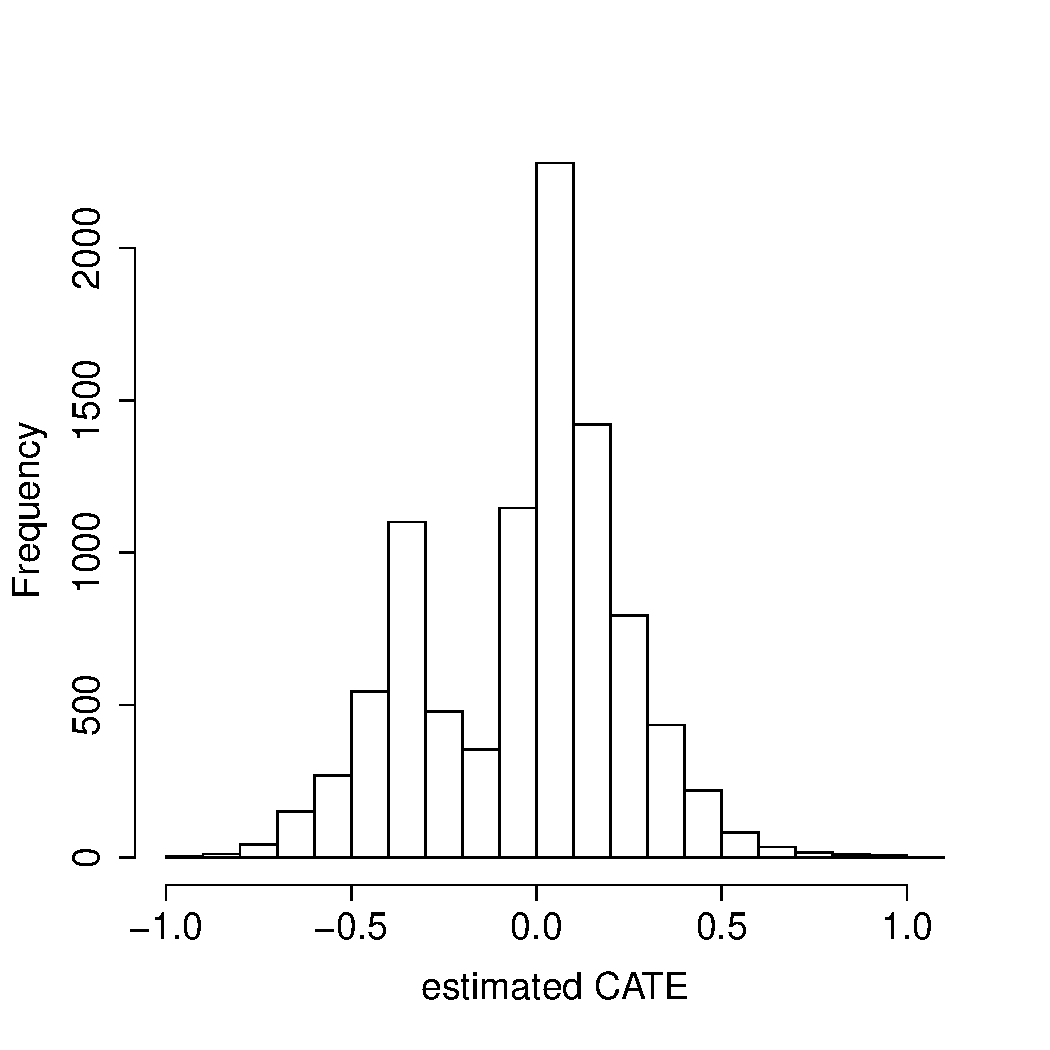
\includegraphics[scale=0.3]{figures/tauhat3_ama_hist.pdf}
    \caption{ Histogram of out-of-bag CATE estimates from a causal forest}
    \label{fig:tauhat3_ama_hist}
\end{figure}
 \end{column}

 \begin{column}{.39\textwidth}
 \begin{table}[h]
 \caption{95\% CI for the ATT} 
\centering
\begin{tabular}{rrr}
  \hline
  2.5\%  & $\hat{\tau_t}$ & 97.5\% \\ 
  \hline
 0.02 & 0.27 & 0.52 \\ 
   \hline
\end{tabular}
\end{table}
 \end{column}
\end{columns}
\end{frame}

\begin{frame}{on bestbuy.com Pages Per Dollar of Sales}
% The first question asks about the overall effectiveness of the intervention. 
\vspace{-1em}
\begin{columns}
\begin{column}{.6\textwidth}
 \begin{figure}[h]
    \centering
    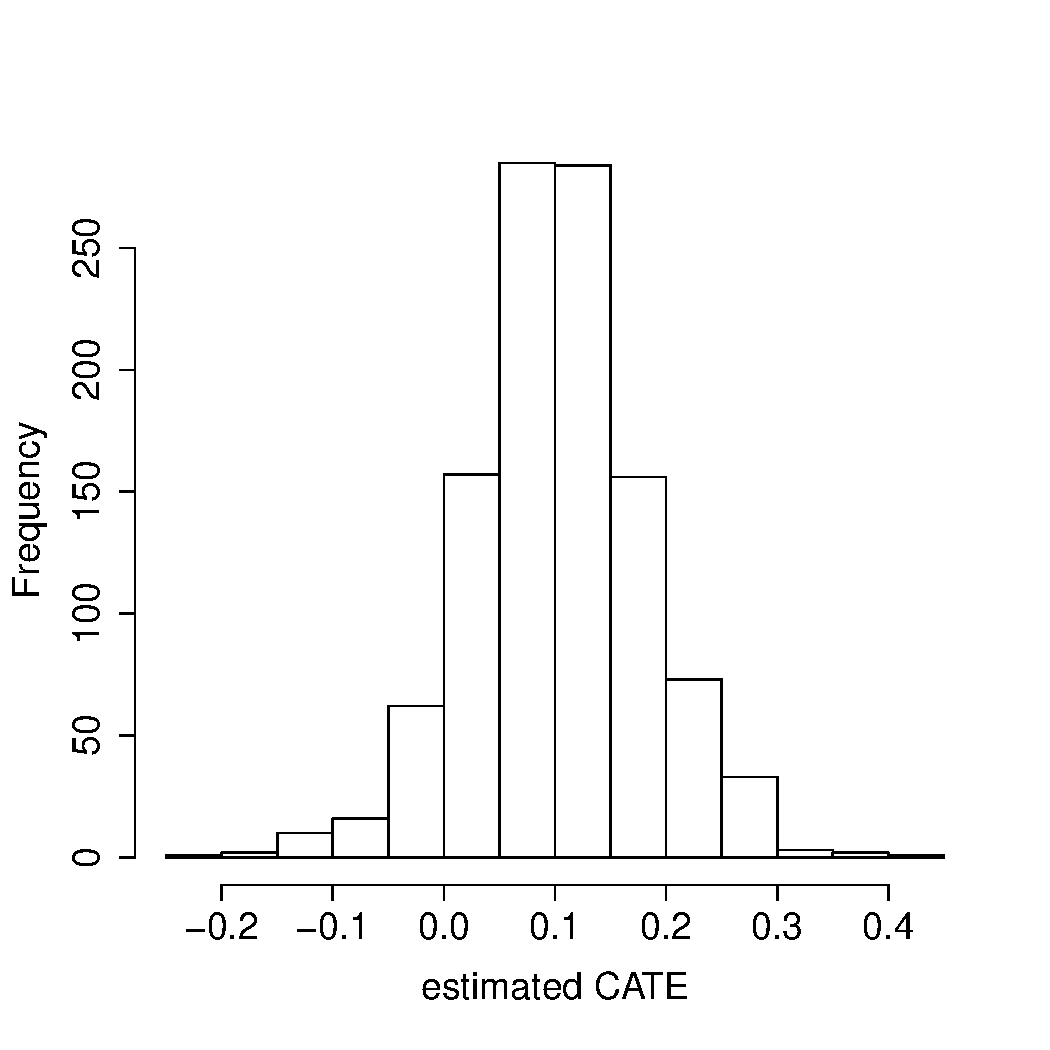
\includegraphics[scale=0.3]{figures/tauhat3_bb_hist.pdf}
    \caption{ Histogram of out-of-bag CATE estimates from a causal forest}
    \label{fig:tauhat3_bb_hist}
\end{figure}
 \end{column}
 
 \begin{column}{.39\textwidth}
\begin{table}[h]
\caption{90\% CI for the ATT} 
\centering
\begin{tabular}{rrr}
  \hline
 5\%  & $\hat{\tau_t}$ & 95\% \\ 
  \hline
 -0.47 & 0.09 & 0.65 \\ 
   \hline
\end{tabular}
\end{table}
 \end{column}
\end{columns}
\end{frame}

\begin{frame}{on amazon.com Minutes Per Dollar of Sales}
% The first question asks about the overall effectiveness of the intervention. 
\vspace{-1em}
\begin{columns}
\begin{column}{.6\textwidth}
 \begin{figure}[h]
    \centering
    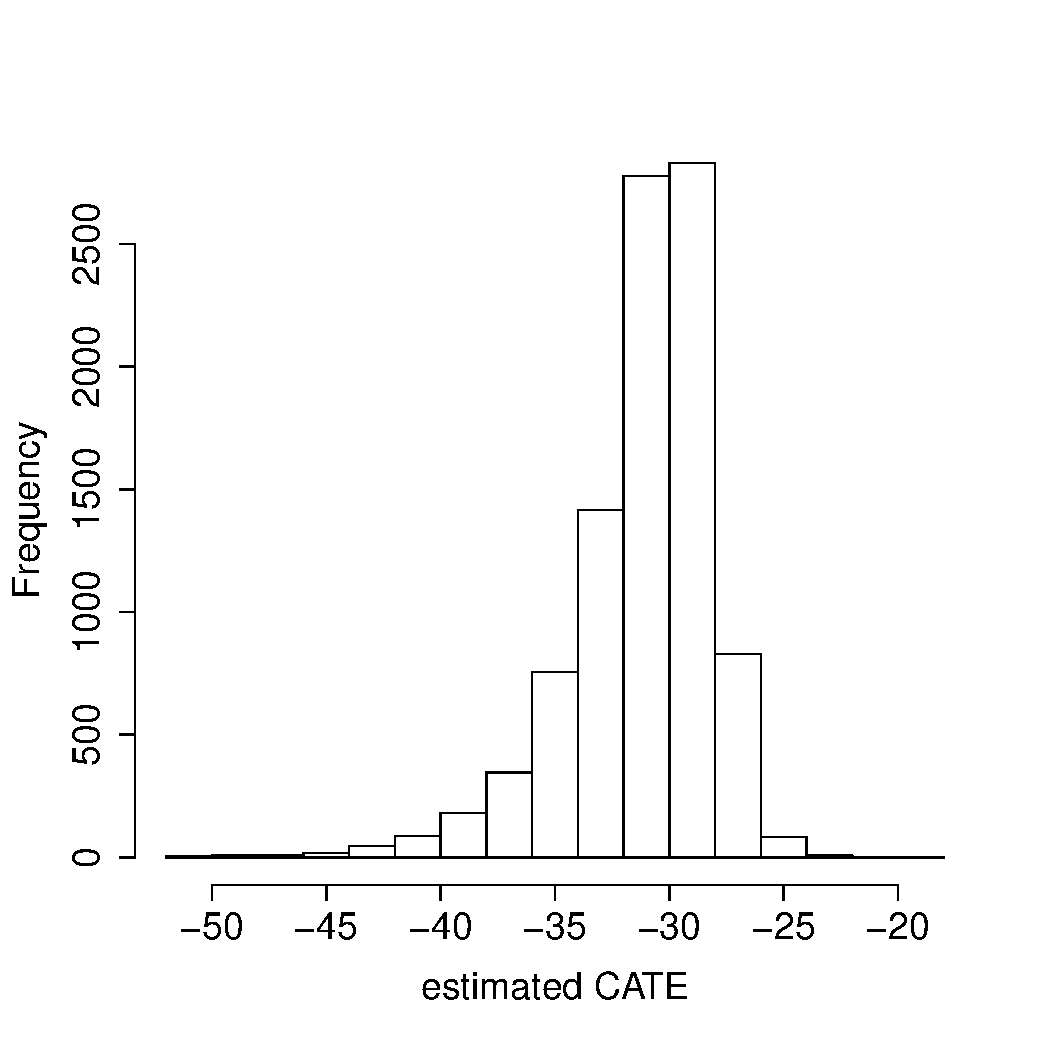
\includegraphics[scale=0.3]{figures/tauhat5_ama_hist.pdf}
    \caption{ Histogram of out-of-bag CATE estimates from a causal forest}
    \label{fig:tauhat5_ama_hist}
\end{figure}
 \end{column}

 \begin{column}{.39\textwidth}
 \begin{table}[h]
 \caption{90\% CI for the ATT} 
\centering
\begin{tabular}{rrr}
  \hline
5\%  & $\hat{\tau_t}$ & 95\% \\ 
  \hline
-110.76 & -24.32 & 62.13 \\ 
   \hline
\end{tabular}
\end{table}
 \end{column}
\end{columns}
\end{frame}

\begin{frame}{on bestbuy.com Minutes Per Dollar of Sales}
% The first question asks about the overall effectiveness of the intervention. 
\vspace{-1em}
\begin{columns}
\begin{column}{.6\textwidth}
 \begin{figure}[h]
    \centering
    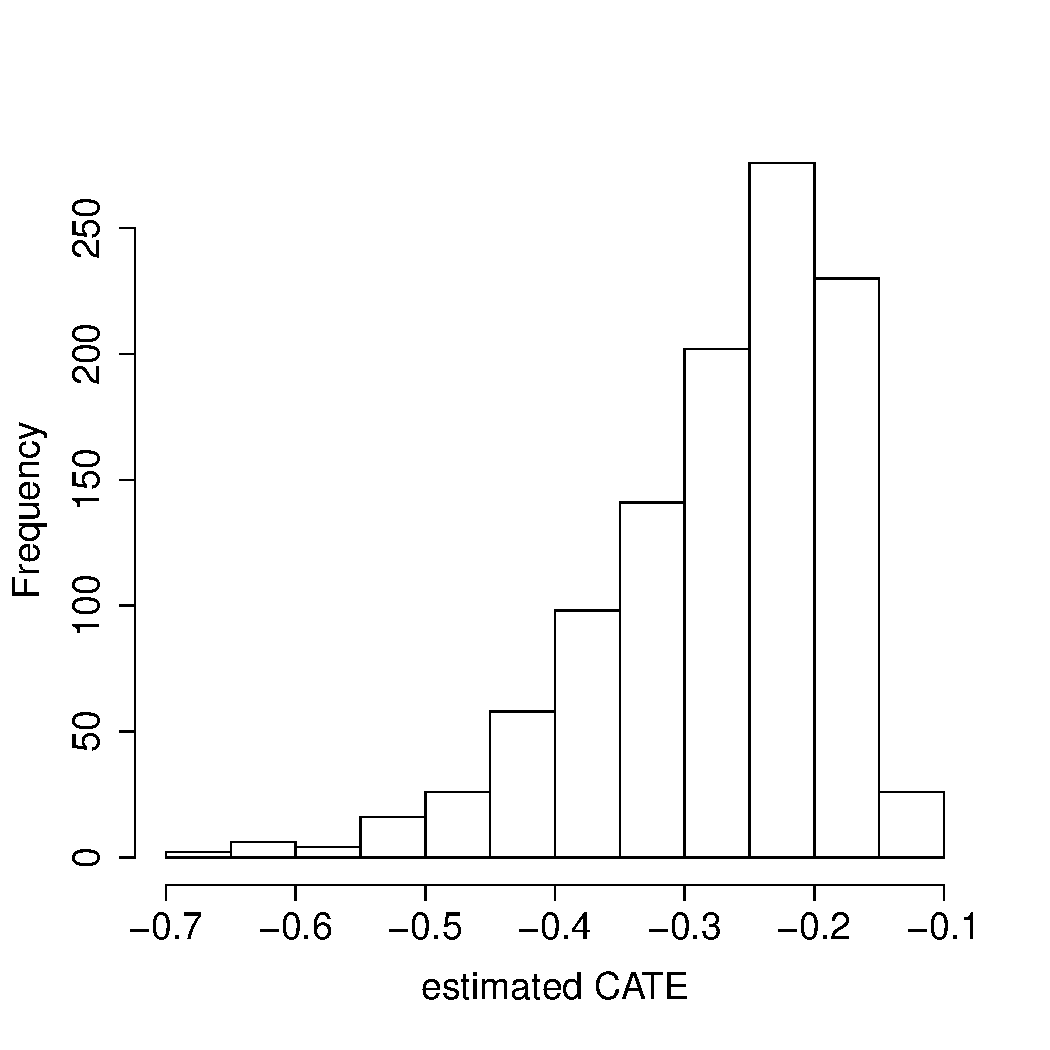
\includegraphics[scale=0.3]{figures/tauhat5_bb_hist.pdf}
    \caption{ Histogram of out-of-bag CATE estimates from a causal forest}
    \label{fig:tauhat5_bb_hist}
\end{figure}
 \end{column}
 
 \begin{column}{.39\textwidth}
\begin{table}[h]
\caption{90\% CI for the ATT}
\centering
\begin{tabular}{rrr}
  \hline
5\%  & $\hat{\tau_t}$ & 95\% \\ 
  \hline
 -0.63 & -0.29 & 0.05 \\ 
   \hline
\end{tabular}
\end{table}
 \end{column}
\end{columns}
\end{frame}


% [allowframebreaks]
\begin{frame}{Reference}
	\bibliography{bobo}
	\bibliographystyle{plainnat}
\end{frame}

\end{document}